\documentclass[hyperref=colorlinks]{beamer}
\mode<presentation>
\usetheme{iclpt}
\setbeamertemplate{navigation symbols}{}
\setbeamertemplate{headline}{
\begin{beamercolorbox}[leftskip=.2cm,rightskip=.2cm,topskip=.2cm,ht=1.1cm,dp=0.1cm,wd=\textwidth]{institute in head/foot}
  
\includegraphics[height=1cm]{icl.pdf}
  \hfill
  
\includegraphics[height=1cm]{../Pics/CMS-Color.pdf}
\end{beamercolorbox}
}
\setbeamertemplate{footline}{
\begin{beamercolorbox}[ht=.55cm,dp=0.4cm,wd=\textwidth,leftskip=.3cm]{author in head/foot}%
  \begin{minipage}[c]{5cm}%
    \usebeamerfont{author in head/foot}
    \insertshortauthor 
    \insertshorttitle
    \end{minipage}\hfill%
  \insertframenumber{} / \pageref{lastframe}
  \hfill
  \begin{minipage}{6cm}
    \hfill
  \end{minipage}
\end{beamercolorbox}%
}

\usepackage{color}
\usepackage{tabularx,colortbl}
\usepackage{graphicx}
\usepackage{pdfpages}
\usepackage{feynmp}
\DeclareGraphicsRule{*}{mps}{*}{}

\title{\vspace{-0.2cm} Combination of Invisible Higgs Direct Measurements}
\subtitle{Paper - HIG-13-030, PASs: HIG-13-013, HIG-13-018, HIG-13-028 \vspace{-0.7cm}}
\author[P. Dunne]{\underline{P. Dunne} \\ on behalf of the H$\rightarrow$invisible analysis groups} % A.M. Magnan and A. Nikitenko Joao Pela with \\ R. Aggleton, J. Brooke: Bristol \\ C.Asawangtrakuldee, Q.Li: Peking \\ P. Srimanobhas: Chulalongkorn \\ S. Kumar, K. Mazumdar: Mumbai}
\titlegraphic{
  \vspace{-0.7cm}
  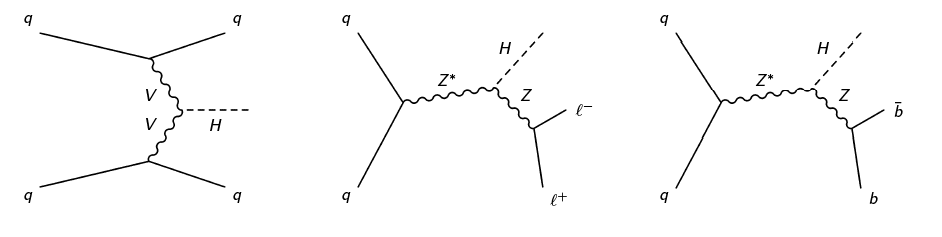
\includegraphics[width=\textwidth]{TalkPics/invcomb021213/feyndiags}
%% \begin{fmfgraph*}(100,70)
%%         \fmfleft{i1,i2}
%%         \fmfright{o1,o2,o3}
%%         \fmf{fermion}{i1,v1,o1}
%%         \fmf{fermion}{i2,v2,o3}
%%         \fmf{phantom,tension=4/5}{v1,v2}
%%         \fmffreeze
%%         \fmf{photon,label=$W,,Z$}{v1,v3}
%%         \fmf{photon,label=$W,,Z$}{v2,v3}
%%         \fmf{dashes}{v3,o2}
%%         \fmflabel{$q$}{i1}
%%         \fmflabel{$q$}{i2}
%%         \fmflabel{$q$}{o1}
%%         \fmflabel{$q$}{o3}
%%         \fmflabel{$H$}{o2}
%%       \end{fmfgraph*}
}
\date{}
\begin{document}
\begin{fmffile}{hig1330approvalfeynmandiags}

%TITLE PAGE
\section{Title}
\begin{frame}
  \titlepage
  
\end{frame}

\begin{frame}
  \begin{columns}
    \column{.35\textwidth}
    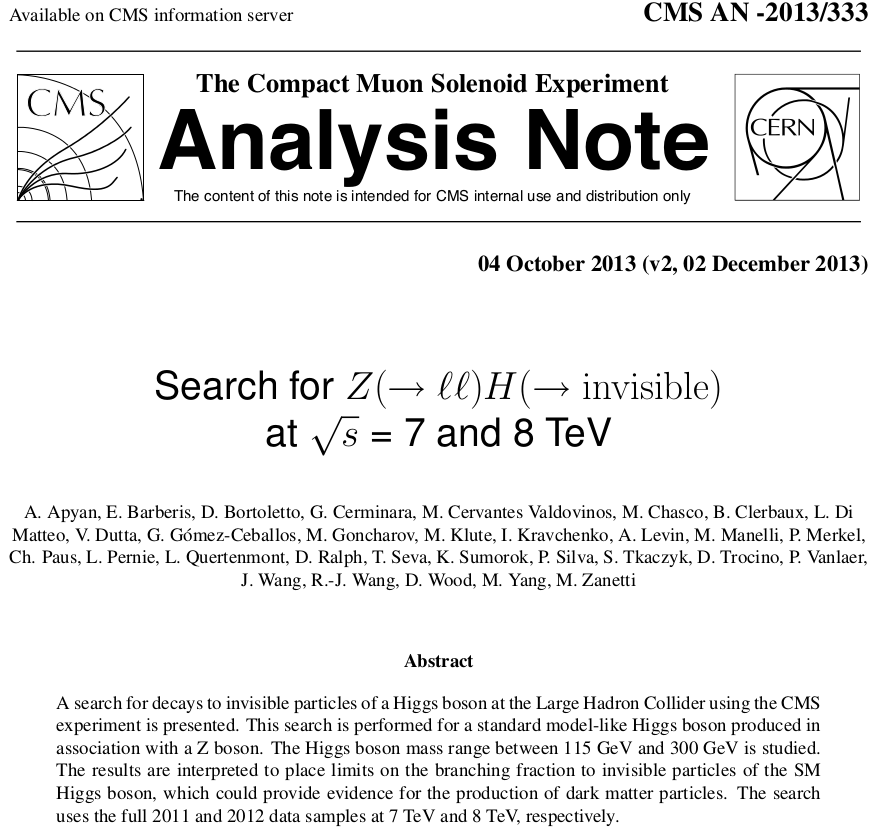
\includegraphics[width=\textwidth]{TalkPics/hig1330approval/zllan}
    \column{.35\textwidth}
    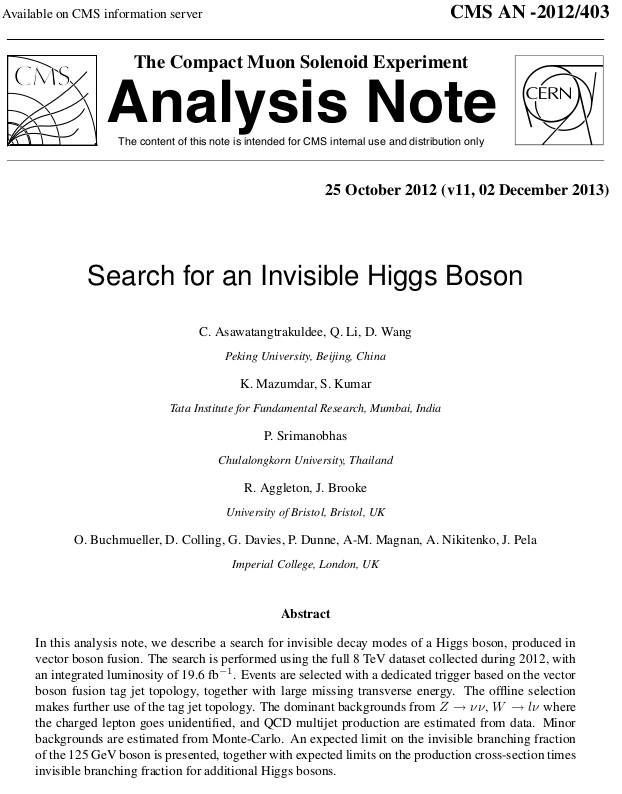
\includegraphics[width=\textwidth]{TalkPics/hig1330approval/vbfan}
    \column{.35\textwidth}
    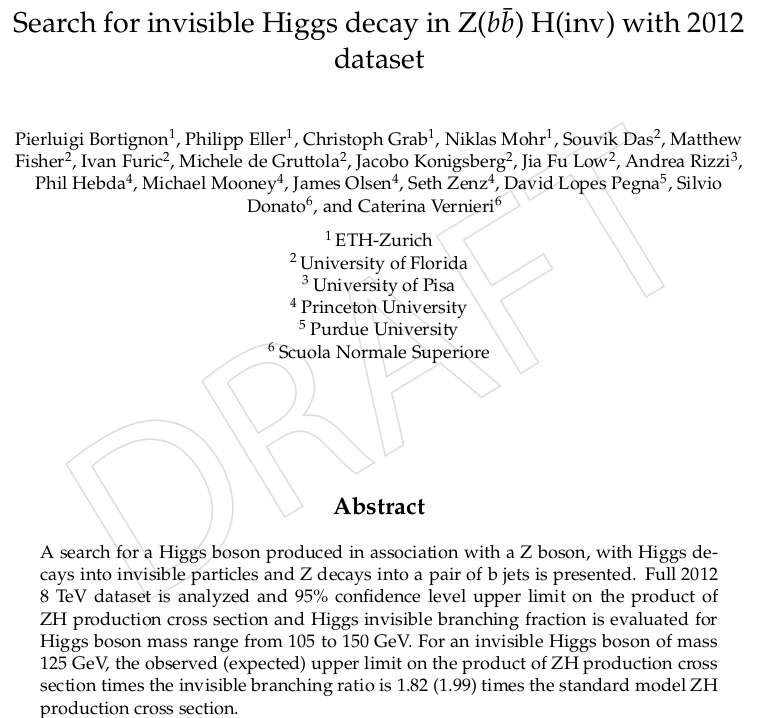
\includegraphics[width=\textwidth]{TalkPics/hig1330approval/zbban}
  \end{columns}
\end{frame}

%OUTLINE
\begin{frame}
  \frametitle{Introduction}
  \begin{block}{\scriptsize Motivation}
    \scriptsize
  \begin{itemize}
  \item Many BSM theories predict invisible final states of the Higgs:
  \item[-] SUSY, Extra Dimensions, etc.
  \item Direct searches must be performed in channels where the Higgs recoils against a visible system
    \end{itemize}
    \end{block}
  \begin{block}{\scriptsize Outline}
    \scriptsize
    \begin{itemize}
  \item The CMS Higgs to invisible results in the following three channels have already been approved:
  \item[-] VBF (HIG-13-013), Z($\ell\ell$)H(inv) (HIG-13-018), Z($b\bar{b}$)H(inv) (HIG-13-028)
  \item These results have been combined for a paper (HIG-13-030)
  \item Today's talk is an approval for this combination and its interpretation in a Higgs portal dark matter model.
  \end{itemize}
  \end{block}
\end{frame}

\begin{frame}
  \frametitle{Indirect Result from Visible Decays}
  \centering

  \vspace{-.2cm}

  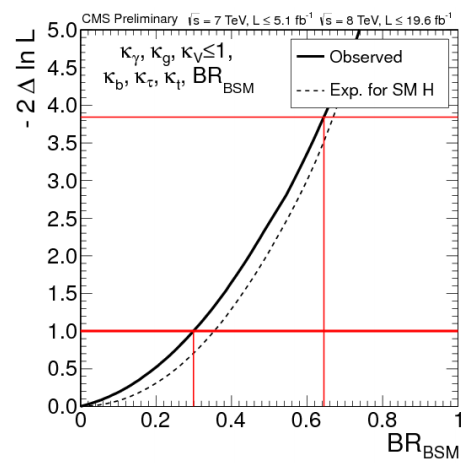
\includegraphics[height=.6\textheight]{indirectbrbsm.png}
  \vspace{-.2cm}

  From HIG-13-005
  \begin{block}{}
    \scriptsize
  \begin{itemize}
  \item Observed (expected) limit of 64\% (67\%) at 95\% C.L. on $BR_{inv} $ for a 125 GeV Higgs (HIG-13-005)
  \item[-] Combination between direct and indirect methods is being investigated e.g. \href{https://indico.cern.ch/getFile.py/access?contribId=3&sessionId=9&resId=1&materialId=slides&confId=267834}{talk by M. Zanetti}
  \end{itemize}
  \end{block}
\end{frame}

\begin{frame}
  \frametitle{Datacards}
  \begin{block}{}
    \scriptsize
  \begin{itemize}
    \item All three channels have signal MC at different mass points
  \end{itemize}
  \end{block}
  \begin{center}
  \begin{tabular}{|l|c|}
    \hline
    Channel & Mass Points/GeV \\
    \hline
    Z($\ell\ell$)H(inv) & 105, 115, 125, 135, 145, 175, 200 \& 300 \\
    Z($b\bar{b}$)H(inv) & 105, 115, 125, 135, 145 \& 150 \\
    VBF & 110, 125, 150, 200, 300 \& 400 \\
    \hline
  \end{tabular}
  \end{center}
  \vspace{-0.3cm}
  \begin{block}{}
   \scriptsize
  \begin{itemize}
  \item New VBF datacards were produced for 115,135 and 145 GeV
  \item[-] Nuisances are linearly interpolated between mass points.
  \item[-] Signal yields are interpolated using the method described below.
  \end{itemize}
  \end{block}
\end{frame}  

\begin{frame}
  \frametitle{Signal Yield interpolation}
  \begin{columns}
    \column{.5\textwidth}
    \begin{block}{}
      \scriptsize
    \begin{itemize}
    \item $N_{Signal}=eff. \times acc. \times \mathcal L\sigma$
    \item Luminosity is constant
    \item Yield over cross-section is thus proportional to efficiency times acceptance
    \item[-] YR2 cross-sections from LHC-HXSWG were used
    \end{itemize}
    \end{block}
    \column{.5\textwidth}
    \centering
    \hspace{-.5cm}
    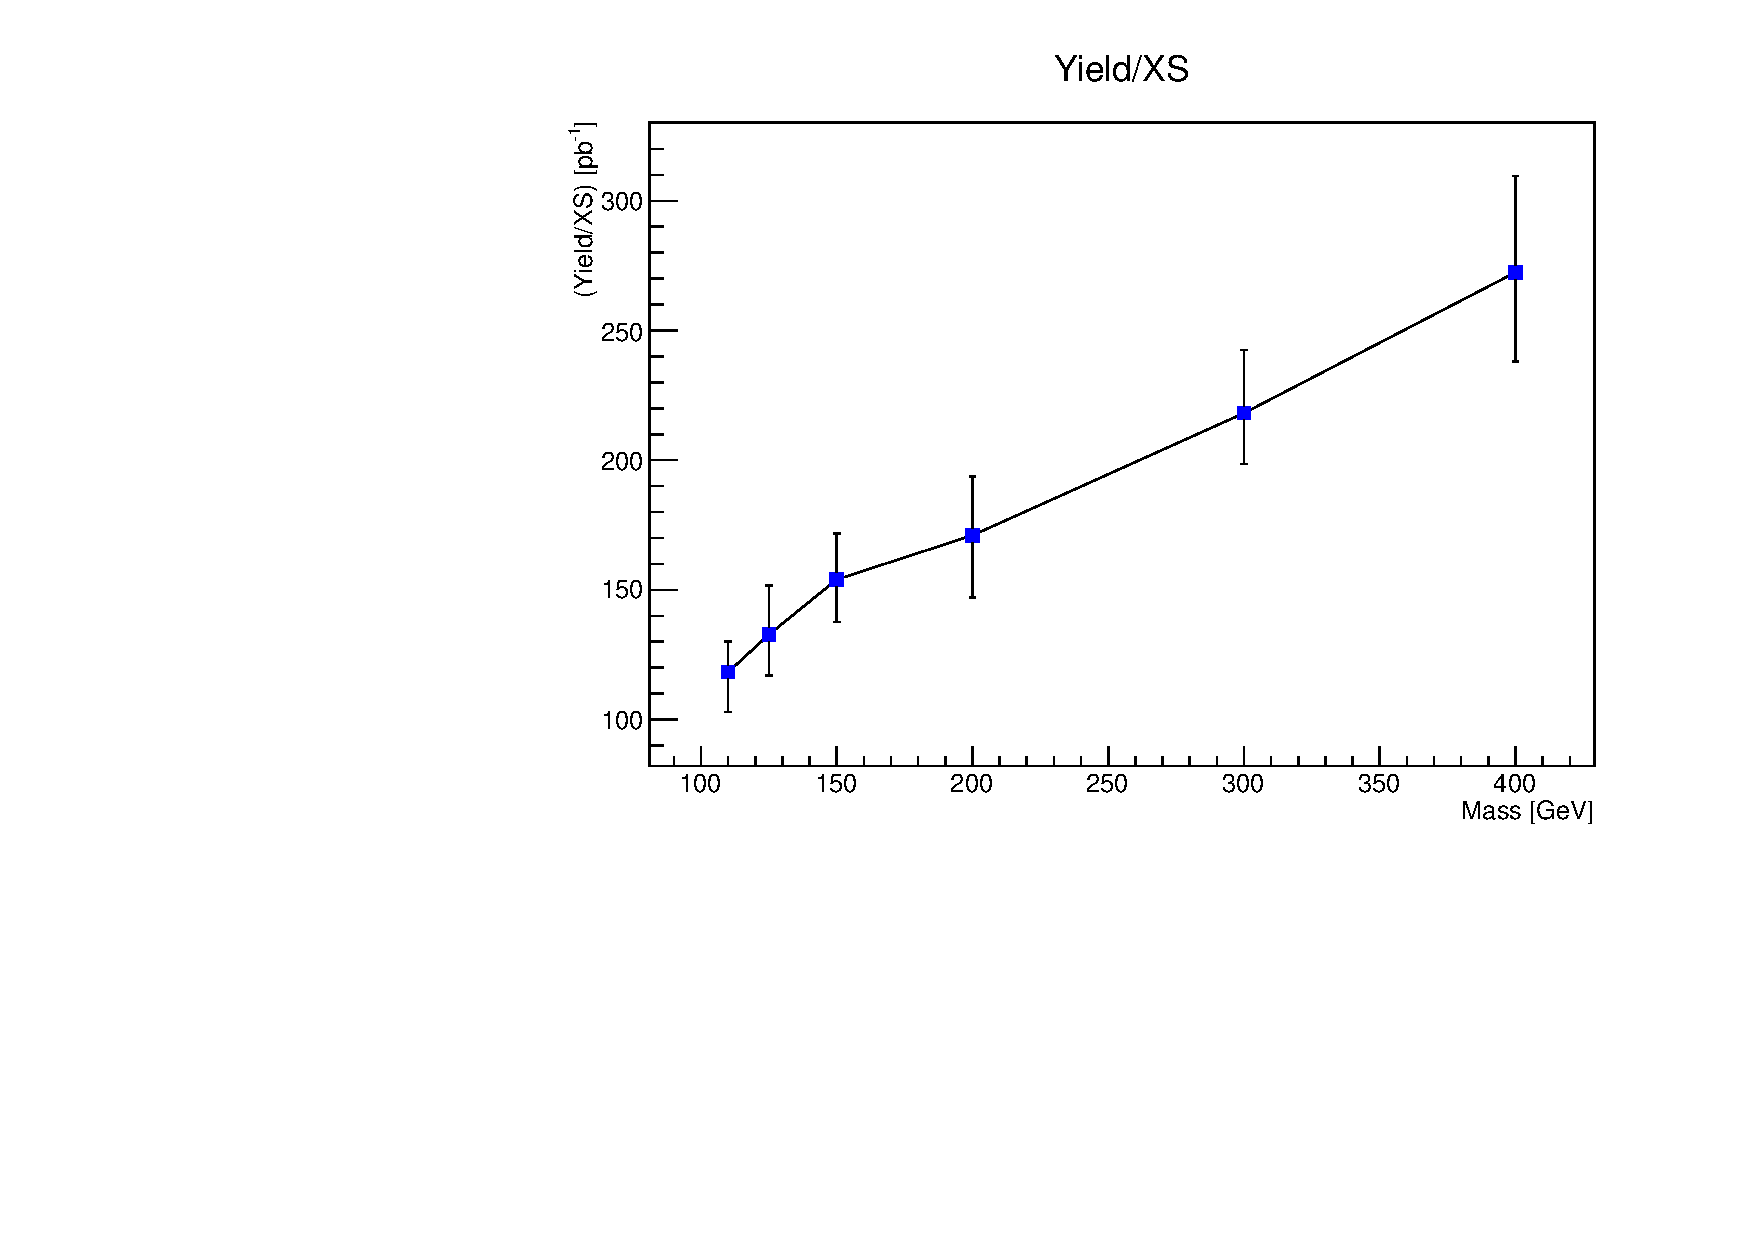
\includegraphics[clip=true,trim=0 0 0 30, width=1.2\textwidth]{TalkPics/invcomb021213/yieldoverxs.pdf}
  \end{columns}
\end{frame}

\begin{frame}
  \frametitle{Combination Method}
  \begin{block}{}
    \scriptsize
  \begin{itemize}
  \item The cards for the three channels were checked by the combinations group and combined using the standard Higgs combination tool
  \item The following uncertainties were considered correlated between channels in decreasing order of importance:
  \end{itemize}
  \end{block}
  \begin{columns}
    \column{1.15\textwidth}
  \begin{block}{}
         \scriptsize
    \centering
    \begin{tabular}{|l|c|c|}
      \hline
      Nuisance & Analyses which it affects & Limit change on removal \\
      \hline
      Jet energy scale & VBF, Z($\ell\ell$)H(inv) & -5.9\% \\
      PDF uncertainties & VBF, Z($b\bar{b}$), Z($\ell\ell$)H(inv) & -4.2\% \\
      QCD scale & VBF, Z($b\bar{b}$), Z($\ell\ell$)H(inv) & -1.7\%\\
      Luminosity & VBF, Z($b\bar{b}$)H(inv), Z($\ell\ell$)H(inv) & -0.8\%\\
      Jet energy resolution & VBF, Z($\ell\ell$)H(inv) & $<$0.1\%\\
      Unclustered energy scale & VBF, Z($b\bar{b}$)H(inv), Z($\ell\ell$)H(inv) & $<$0.1\%\\
      Muon identification efficiency & VBF, Z($\ell\ell$)H(inv) & $<$0.1\%\\
      Electron identification efficiency & VBF, Z($\ell\ell$)H(inv) & $<$0.1\% \\
      \hline
    \end{tabular}
    \end{block}
  \end{columns}
\end{frame}
    
\begin{frame}
  \frametitle{Separate results: Cross-Section limits}
  \centering
  \begin{columns}
    \column{.5\textwidth}

    \begin{block}{\scriptsize VBF {\color{red} - update of approved plot}}
    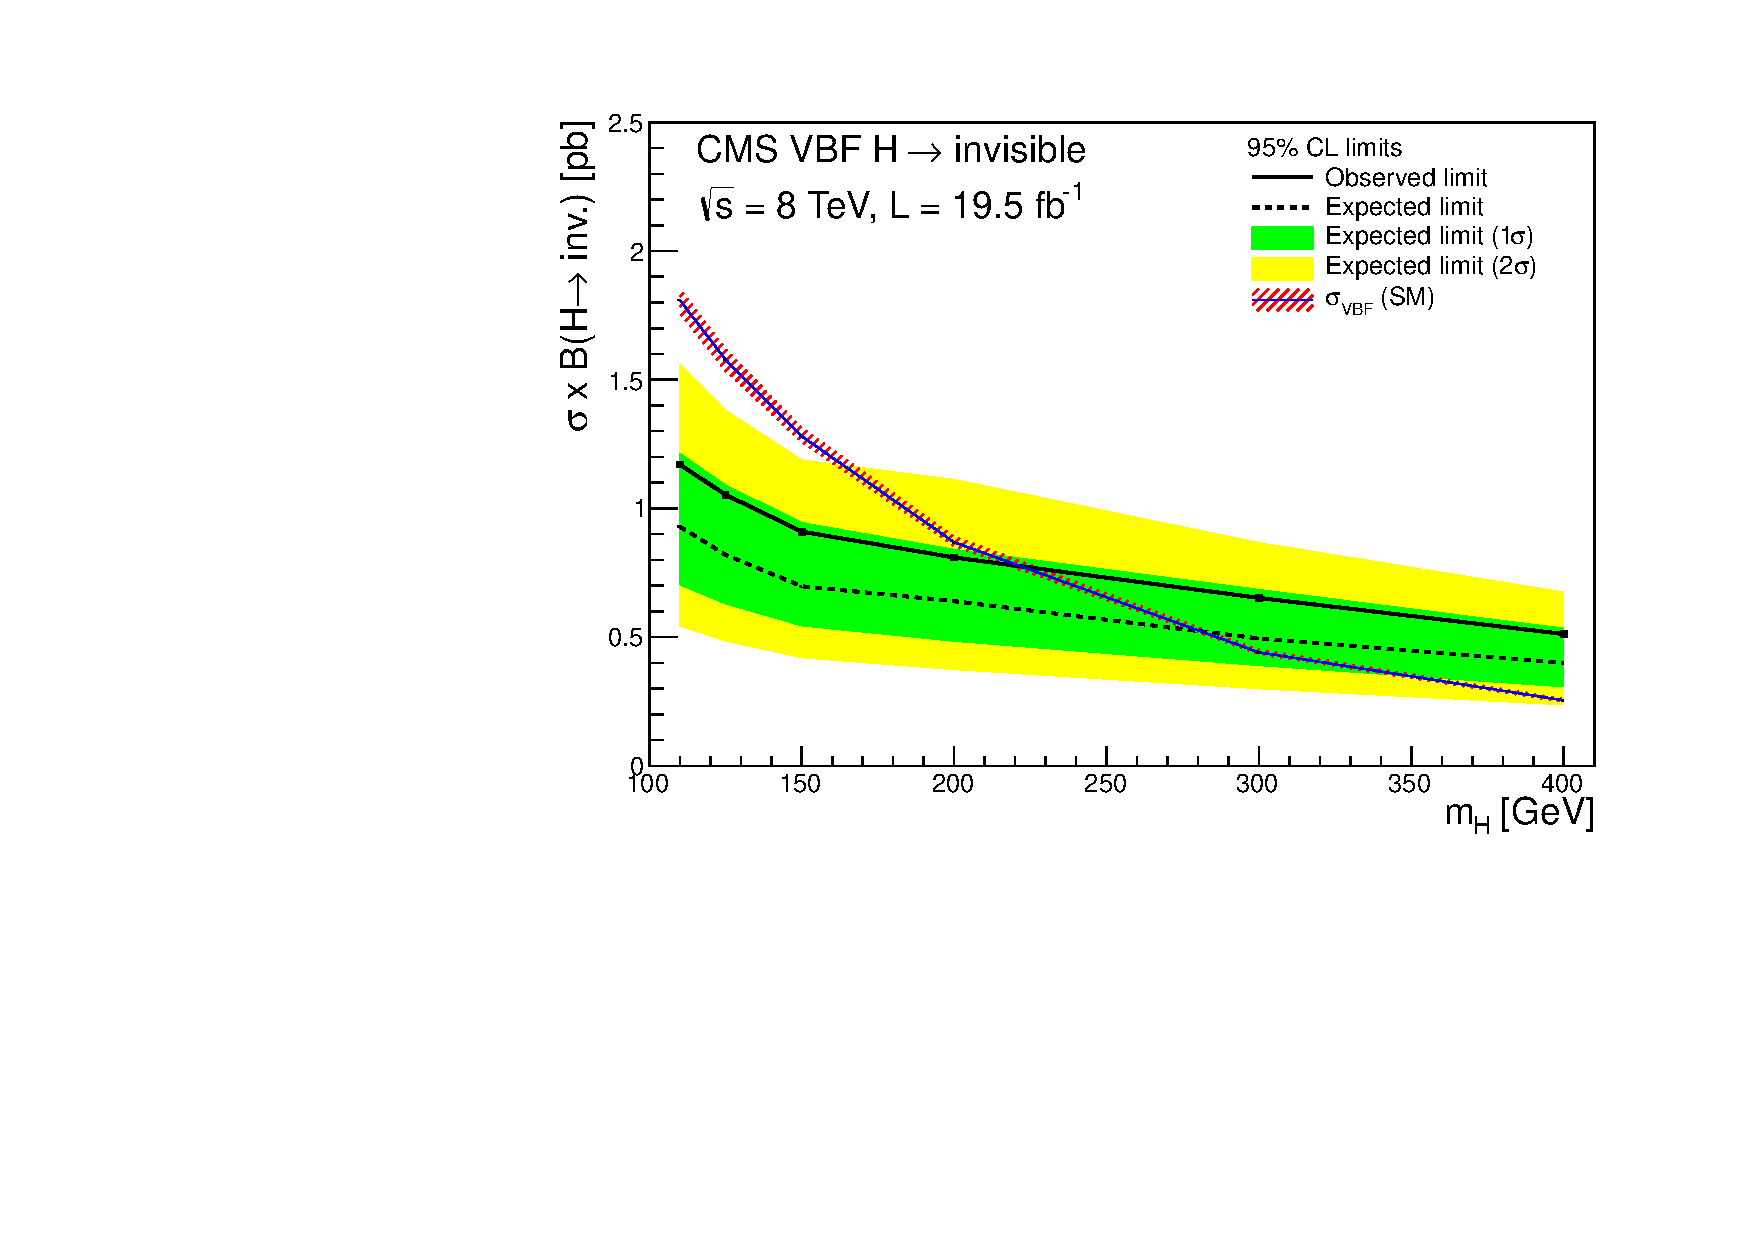
\includegraphics[width=\textwidth]{TalkPics/hig1330approval/vbfxslimit.pdf}
    \scriptsize
    \begin{itemize}
    \item Observed (expected) limit of 67\% (52\%) at 95\% C.L. on $BR_{inv}$ for a 125 GeV Higgs
    \end{itemize}
    
    \end{block}

    \column{.5\textwidth}
    \begin{block}{\scriptsize ZH {\color{red} - for approval}}
      
    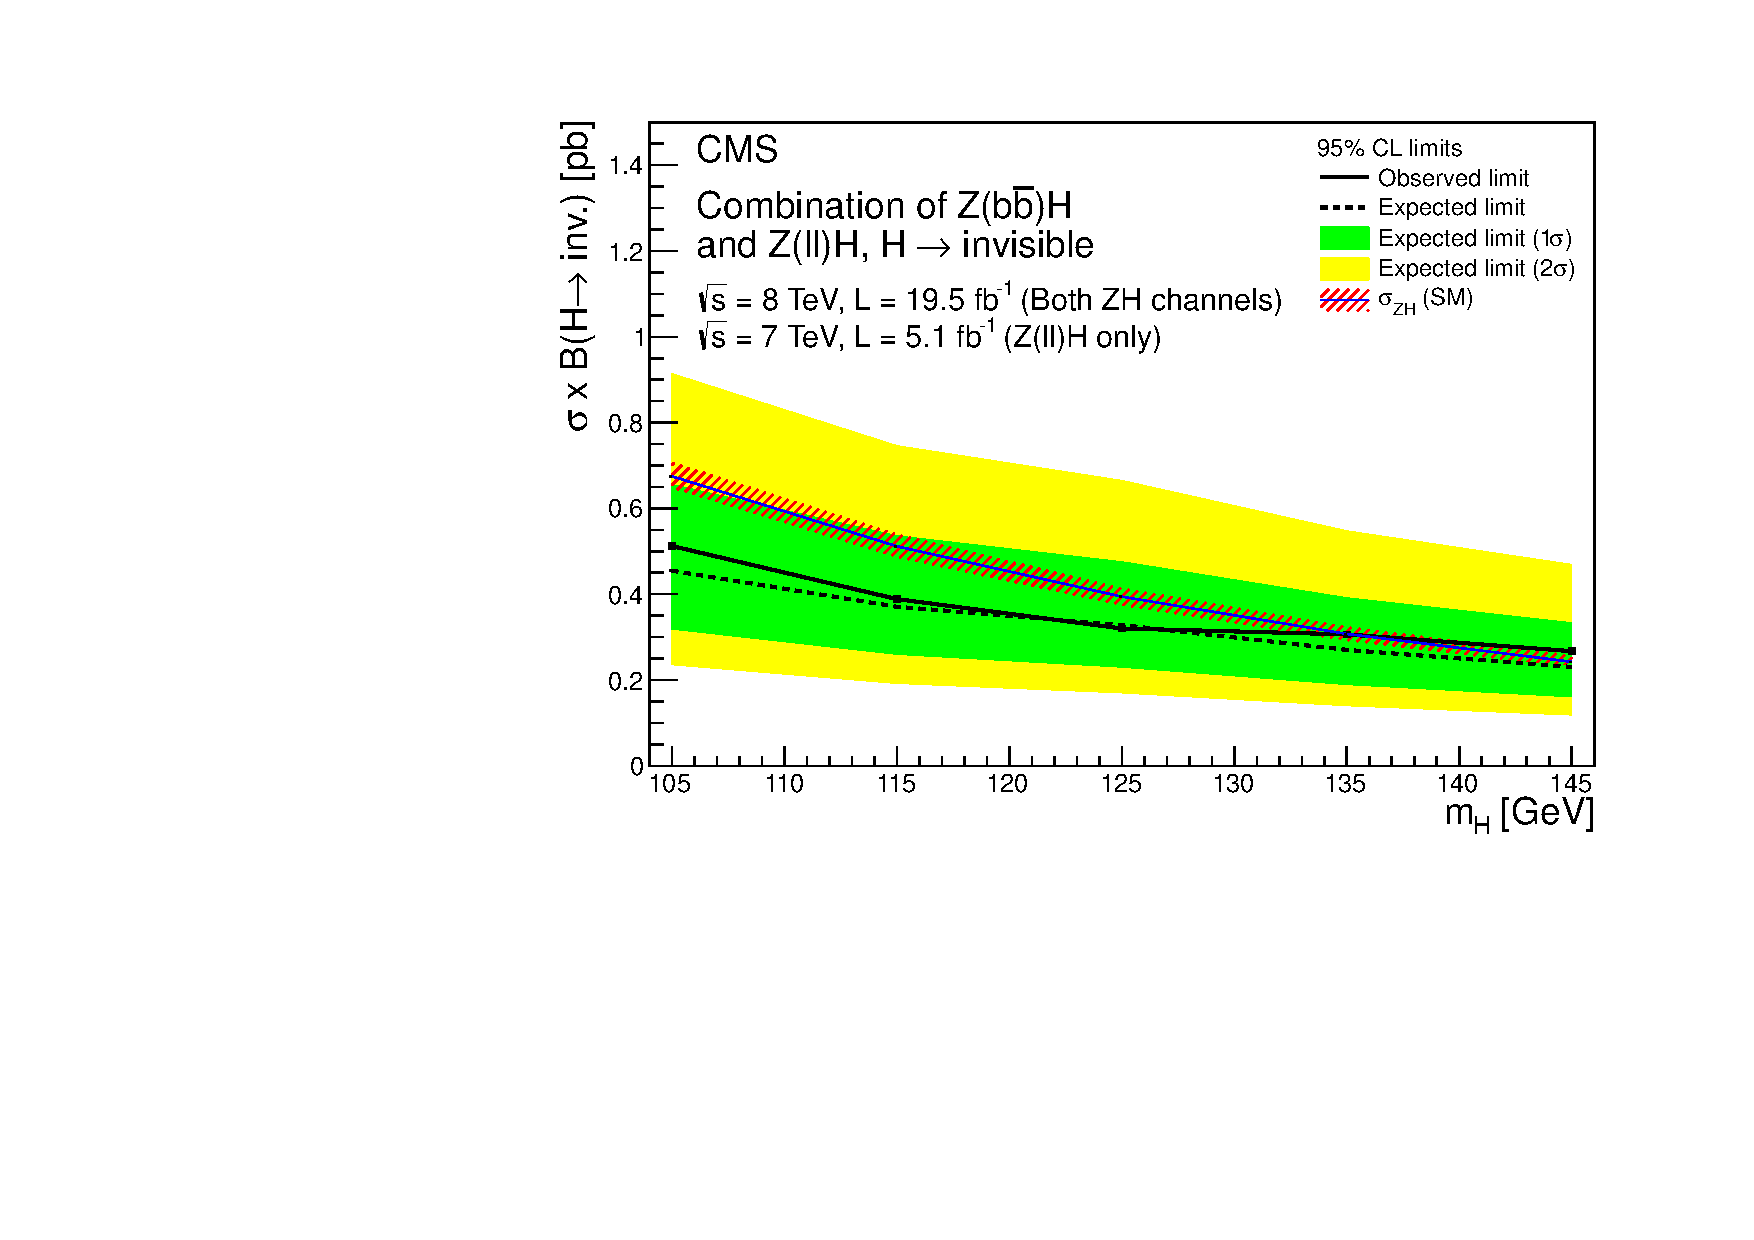
\includegraphics[width=\textwidth]{TalkPics/hig1330approval/zhxslimit.pdf}
    \scriptsize
    \begin{itemize}
    \item Observed (expected) limit of 81\% (83\%) at 95\% C.L. on $BR_{inv}$ for a 125 GeV Higgs
    \end{itemize}

    \end{block}

  \end{columns}

\end{frame}

\begin{frame}
  \frametitle{Separate results: Direct}
  \centering
  \begin{columns}
    \column{.5\textwidth}
    \begin{block}{\scriptsize VBF {\color{red} - update of approved plot}}
    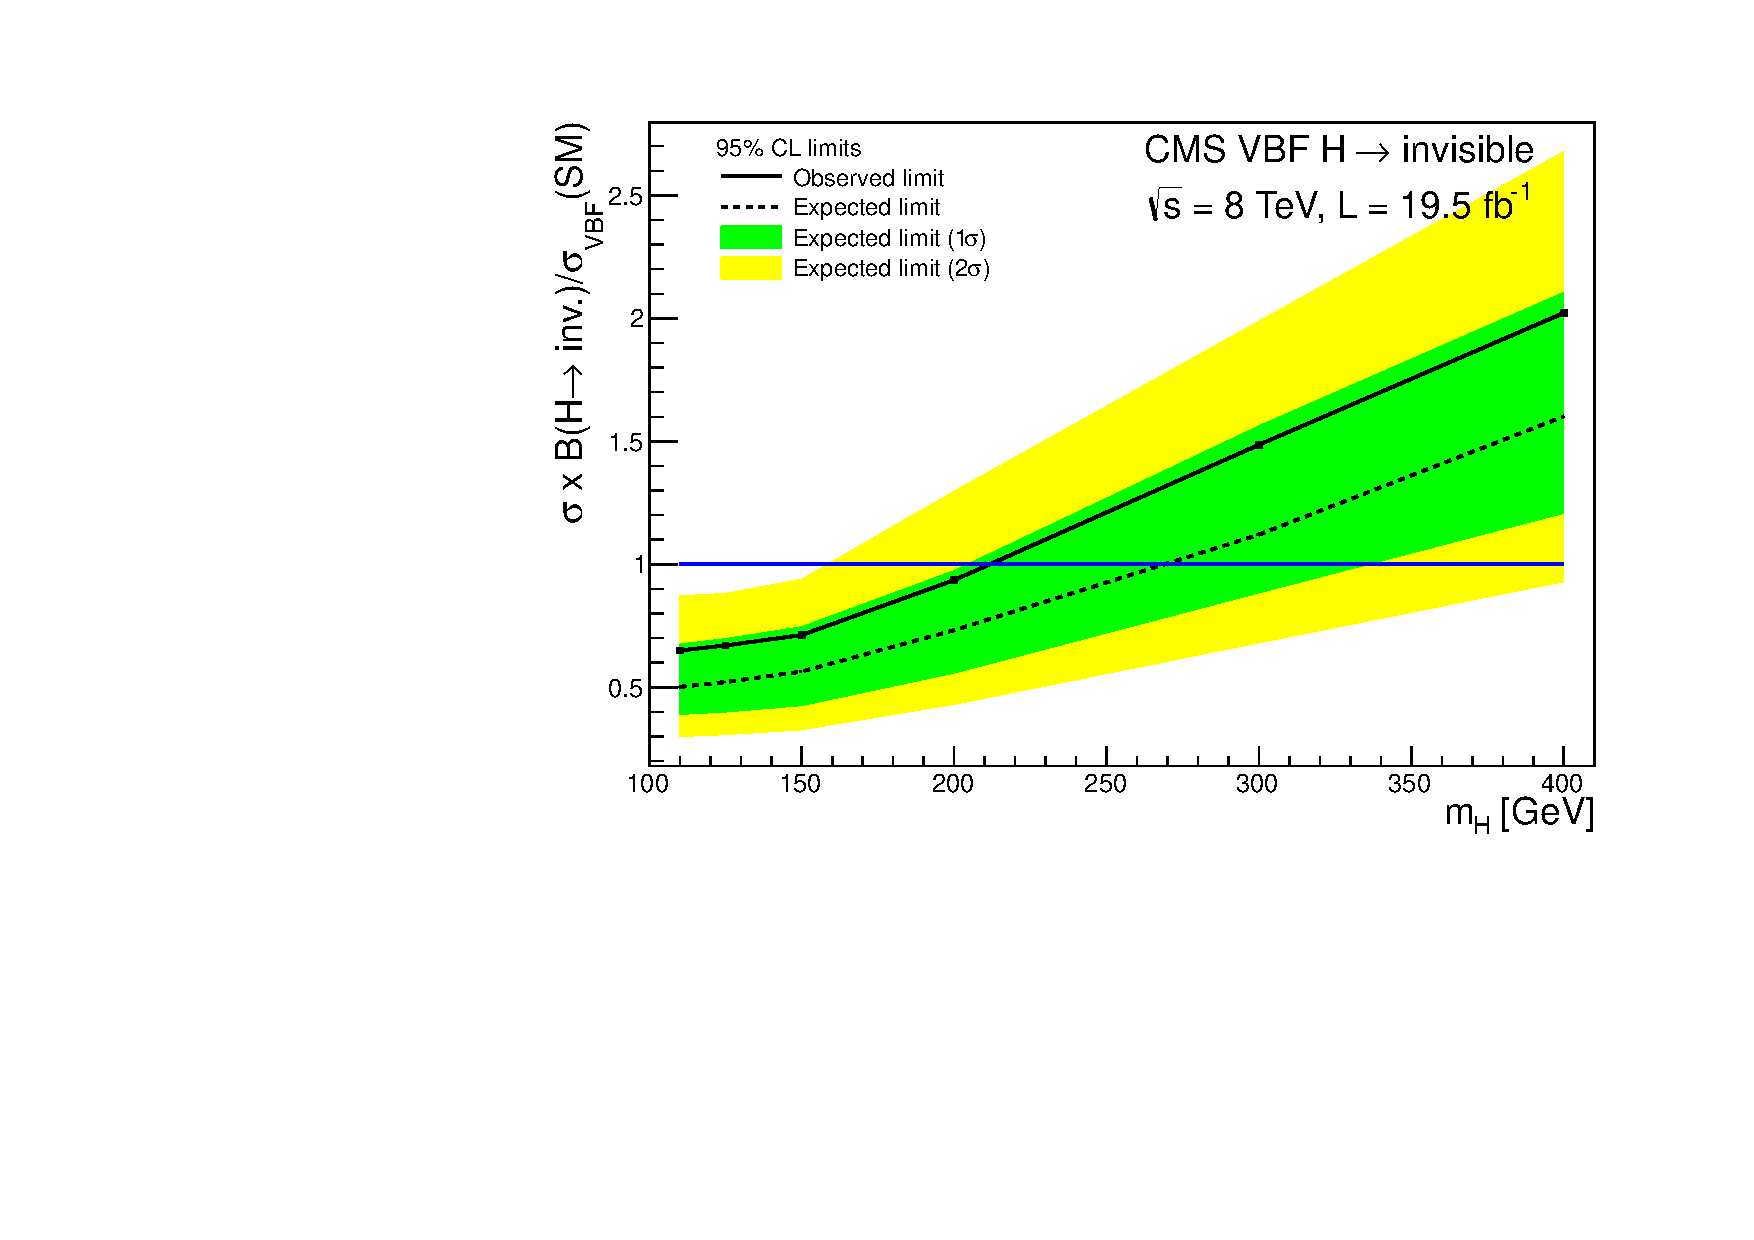
\includegraphics[width=\textwidth]{TalkPics/hig1330approval/vbflimit.pdf}
    \scriptsize
    \begin{itemize}
    \item Observed (expected) limit of 67\% (52\%) at 95\% C.L. on $BR_{inv}$ for a 125 GeV Higgs
    \end{itemize}

    \end{block}

    \column{.5\textwidth}

    \begin{block}{\scriptsize ZH {\color{red} - for approval}}

    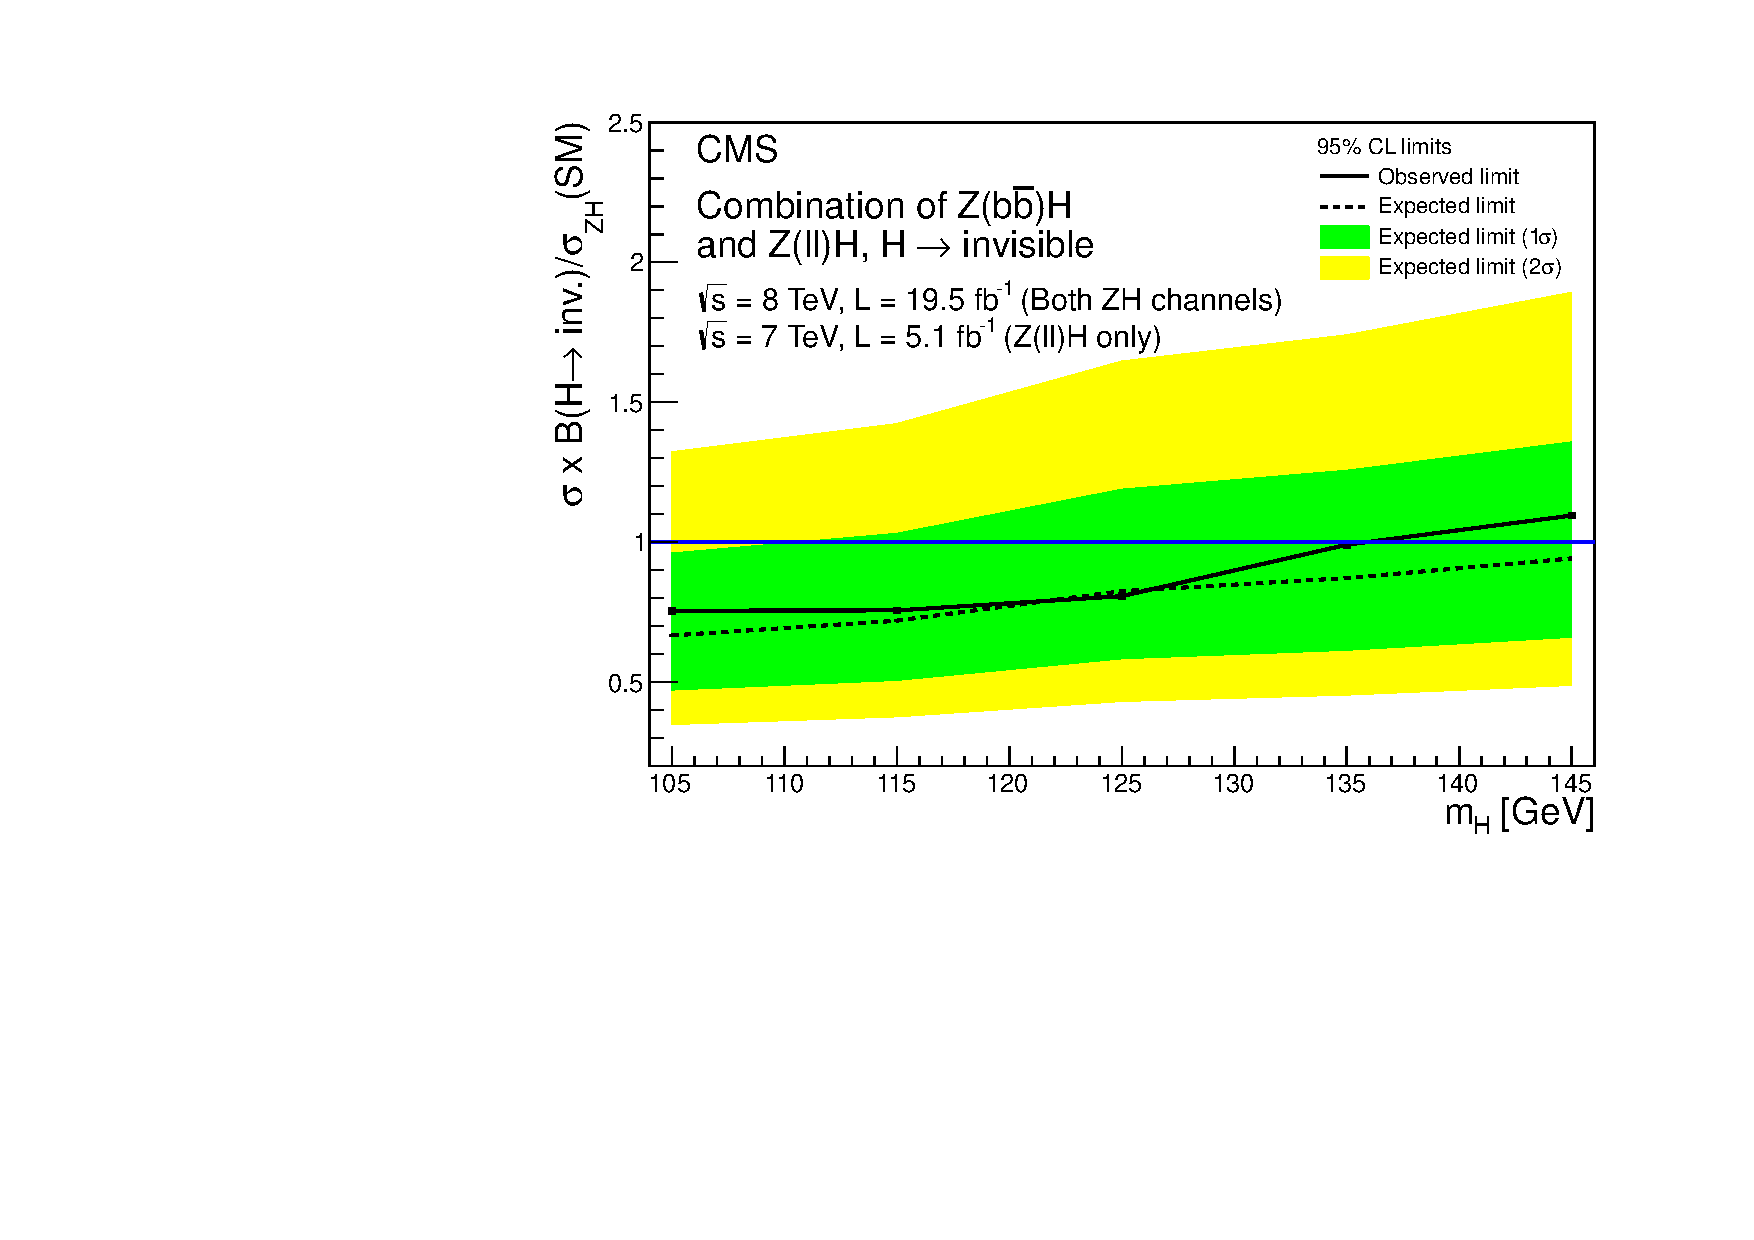
\includegraphics[width=\textwidth]{TalkPics/hig1330approval/zhlimit.pdf}
    \scriptsize
    \begin{itemize}
    \item Observed (expected) limit of 81\% (83\%) at 95\% C.L. on $BR_{inv}$ for a 125 GeV Higgs
    \end{itemize}

    \end{block}

  \end{columns}
\end{frame}



\begin{frame}
  \frametitle{Combined Results}
  \centering

  \vspace{-.2cm}

{\color{red} For approval}



  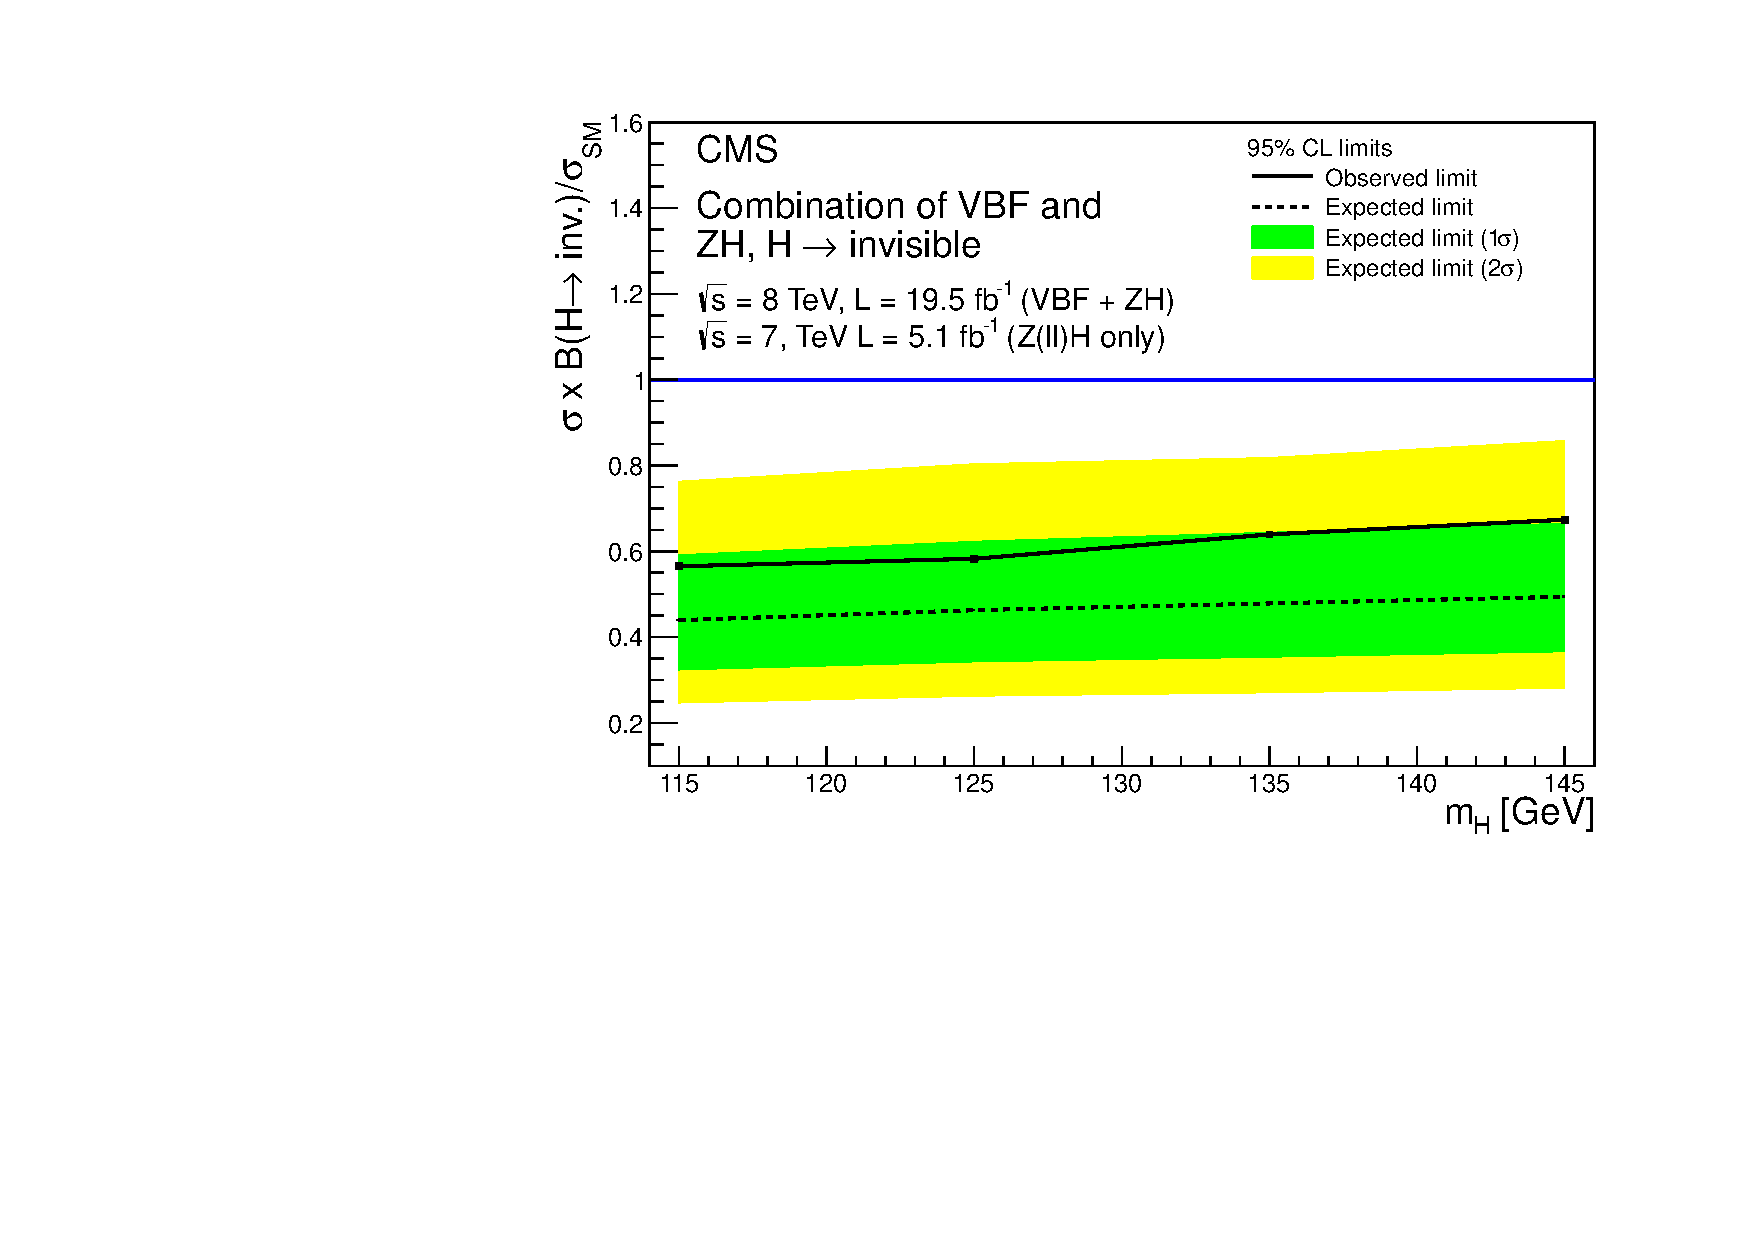
\includegraphics[clip=true,trim=0 0 0 0, width=.75\textwidth]{TalkPics/hig1330approval/combinedlimit.pdf}
  \vspace{-.2cm}
  \begin{block}{}
    \scriptsize
  \begin{itemize}
  \item Observed (expected) limit at 125 GeV is 58(46)\%
  \end{itemize}
  \end{block}
\end{frame}

\begin{frame}
  \frametitle{High mass combination}
  \centering
  \vspace{-.3cm}
  \begin{block}{}
    \footnotesize
  \begin{itemize}
  \item Z($\ell\ell$)H(inv) and VBF both have datacards up to 300 GeV
  \item The same combination method as used above was used to combine these two channels between 115 and 300 GeV
  \end{itemize}
  \end{block}

  \vspace{-.1cm}

  {\color{red} For approval as additional material}
  
  \vspace{-.1cm}
  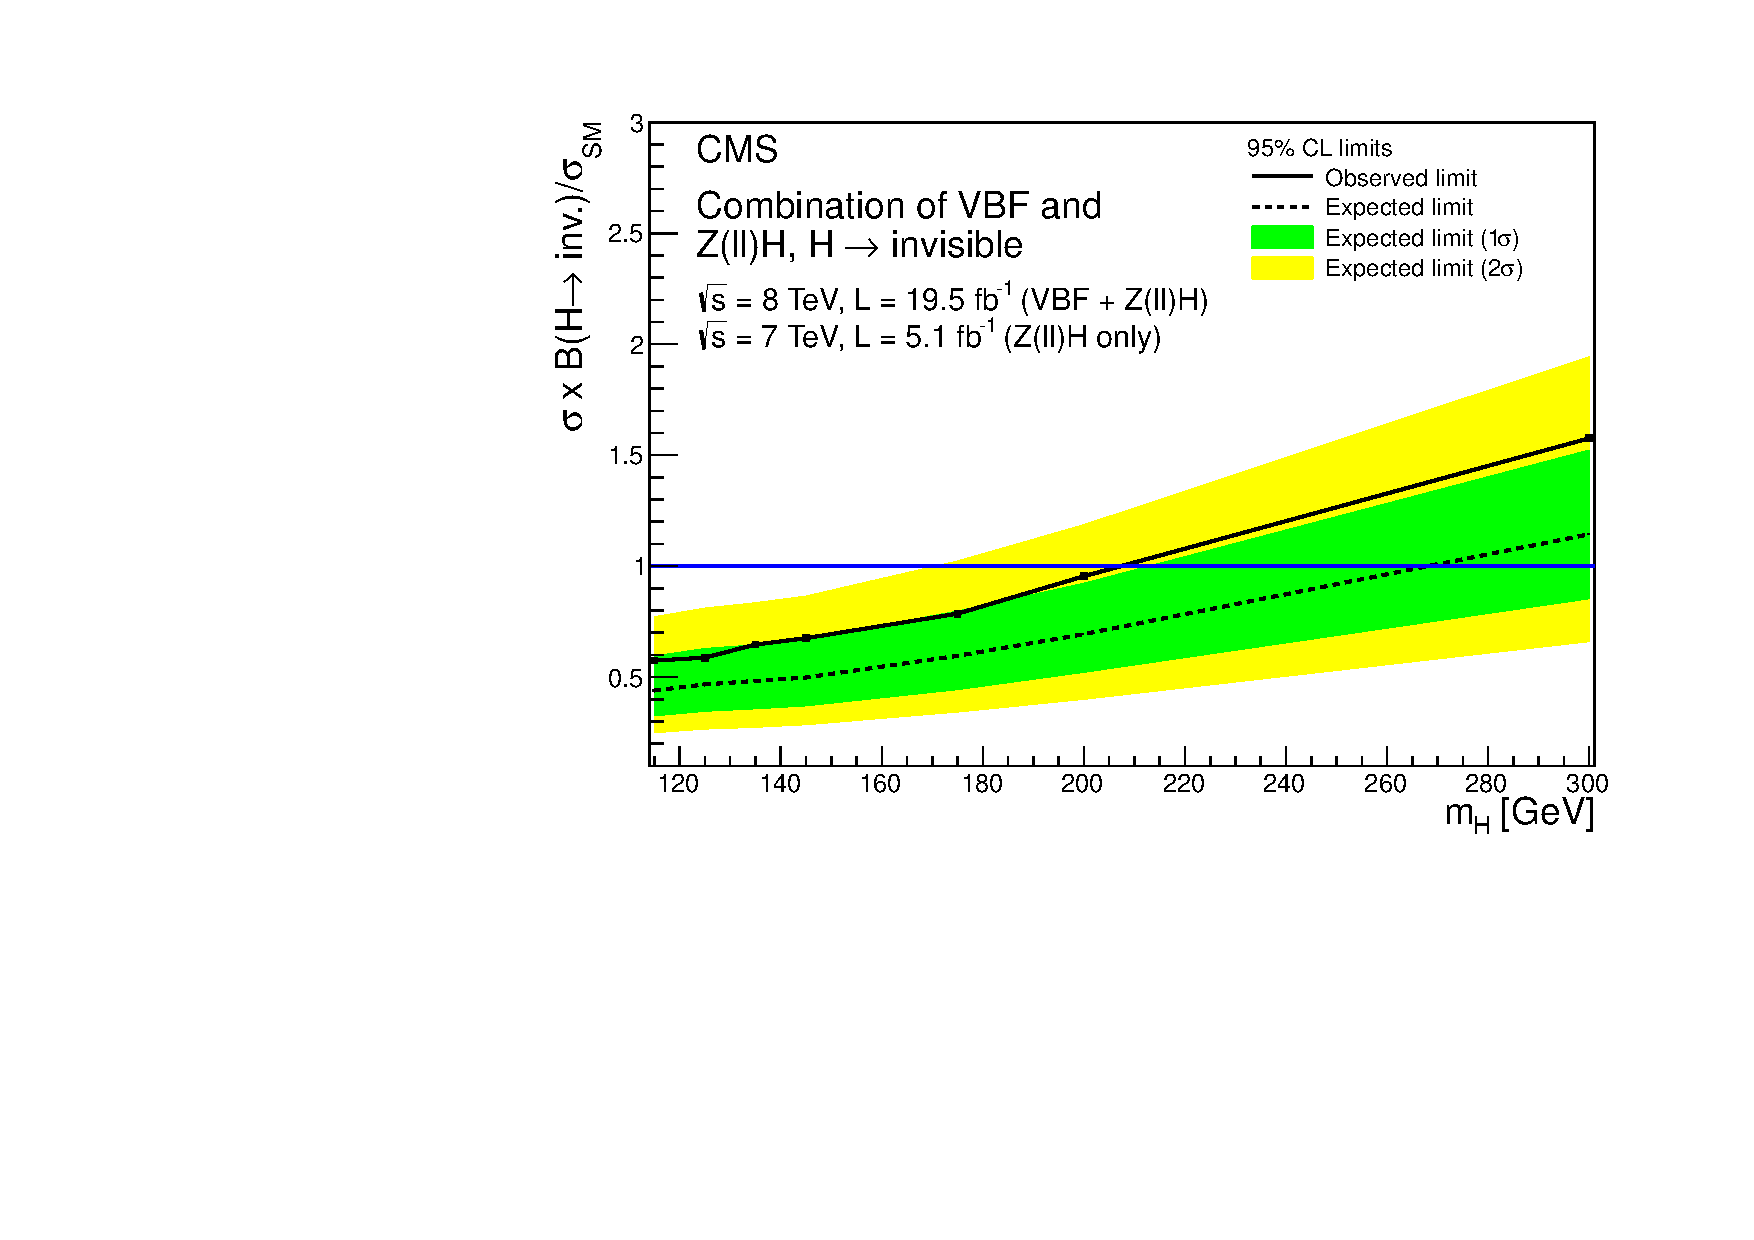
\includegraphics[clip=true,trim=0 0 0 20, width=.68\textwidth]{TalkPics/hig1330approval/highmasslimit.pdf}
\end{frame}

\begin{frame}
  \frametitle{Changes to Plots Since CWR}
  \scriptsize
  \begin{block}{}
  \begin{itemize}
  \item Legends have been made consistent across all combinations plots.
  \item The legend of the final combination plot has been moved further from the blue 'SM' line.
  \item Square brackets are now used for all units.
  \item YR2 Cross-sections are now used where YR3 cross-sections were used before.
  \item Theory uncertainties have been removed from the fit in the $\sigma\mathcal{B}(H\rightarrow inv.)$ plots and a theory uncertainty band has been added to $\sigma_{SM}$.
  \end{itemize}
  \end{block}
\end{frame}


\begin{frame}
  \frametitle{Signatures of Dark Matter (DM)}
  \begin{block}{}
    \scriptsize
    \begin{itemize}
    \item If DM couples to the Higgs the following diagrams are possible
    \end{itemize}
  \end{block}
  \vspace{-.2cm}
  \begin{columns}
    \column{.35\textwidth}
    \begin{block}{\scriptsize Direct Detection - e.g. LUX}
      \vspace{.3cm}
    \begin{fmfgraph*}(100,70)
        \fmfleft{i1,i2}
        \fmfright{o1,o2}
        \fmf{fermion}{i1,v1,o1}
        \fmf{fermion}{i2,v2,o2}
        \fmf{dashes,label=$H$}{v1,v2}
        \fmffreeze
        \fmflabel{$N$}{i1}
        \fmflabel{$\chi$}{i2}
        \fmflabel{$N$}{o1}
        \fmflabel{$\chi$}{o2}
      \end{fmfgraph*}
    \vspace{.3cm}
    \end{block}

    \column{.35\textwidth}
    \begin{block}{\scriptsize Invisible Higgs - LHC}
      \vspace{.3cm}
    \begin{fmfgraph*}(100,70)
        \fmfleft{i1,i2}
        \fmfright{o1,o2}
        \fmf{fermion}{i1,v1,i2}
        \fmf{fermion}{o1,v2,o2}
        \fmf{dashes,label=$H$}{v1,v2}
        \fmffreeze
        %\fmflabel{$f/w/Z$}{i1}
        \fmflabel{$\chi$}{o1}
        %\fmflabel{$f/W/Z$}{i2}
        \fmflabel{$\chi$}{o2}
      \end{fmfgraph*}
    \vspace{.3cm}
    \end{block}
    \column{.35\textwidth}
    \begin{block}{\scriptsize Annihilation - e.g. WMAP}
      \vspace{.3cm}
    \begin{fmfgraph*}(100,70)
        \fmfleft{i1,i2}
        \fmfright{o1,o2}
        \fmf{fermion}{i1,v1,i2}
        \fmf{fermion}{o1,v2,o2}
        \fmf{dashes,label=$H$}{v1,v2}
        \fmffreeze
        %\fmflabel{$f/w/Z$}{i1}
        \fmflabel{$\chi$}{i1}
        %\fmflabel{$f/W/Z$}{i2}
        \fmflabel{$\chi$}{i2}
      \end{fmfgraph*}
    \vspace{.3cm}
    \end{block}
  \end{columns}
  \begin{block}{}
    \scriptsize
    \begin{itemize}
    \item Limits on $\mathcal{B}$(H$\rightarrow$inv.) can therefore be used to constrain the coupling
    \item These constraints are directly comparable to those from other experiments
    \end{itemize}
  \end{block}
\end{frame}

\begin{frame}
  \frametitle{Dark Matter Interpretation - Model}
  \vspace{-.3cm}
  \begin{block}{}
    \scriptsize
    \begin{itemize}
    \item We use the Higgs portal DM model as described in \href{http://www.sciencedirect.com/science/article/pii/S0370269312001037}{Phys.Lett. B709 (2012) 65–69}
    \item This allows us to translate $\mathcal{B}(H\rightarrow inv.)$ to a DM-nucleon cross-section
    \item Three spin scenarios are considered for the DM particle:
    \item[-] scalar, vector, Majorana fermion
    \end{itemize}
  \end{block}
  \vspace{-0.3cm}
  \begin{columns}
    \column{.65\textwidth}
    \begin{block}{\scriptsize Formulae}
      \scriptsize
      \begin{itemize}
      \item $\mathcal{B}(H\rightarrow inv.) = \frac{\Gamma(H \rightarrow inv.)}{\Gamma(H)^{SM}+\Gamma(H\rightarrow inv.)}$
      \item $\sigma^{SI}_{S-N} = \frac{4\Gamma(H \rightarrow inv.)}{m_{H}^{3}v^{2}\beta}\frac{m_{N}^{4}f_{N}^{2}}{(M_{\chi}+m_{N})^{2}}$
      \item $\sigma^{SI}_{V-N} = \frac{16\Gamma(H \rightarrow inv.)M_{\chi}^{4}}{m_{H}^{3}v^{2}\beta(m_{H}^{4}-4M_{\chi}^{2}m_{H}^{2}+12M_{\chi}^{4}}\frac{m_{N}^{4}f_{N}^{2}}{(M_{\chi}+m_{N})^{2}}$
      \item $\sigma^{SI}_{f-N} = \frac{8\Gamma(H \rightarrow inv.)M_{\chi}^{2}}{m_{H}^{5}v^{2}\beta^{3}}\frac{m_{N}^{4}f_{N}^{2}}{(M_{\chi}+m_{N})^{2}} $
        \item[-] Where $f_{N}$ is the Higgs-proton coupling and v is the Higgs vacuum expectation
      \end{itemize}
    \end{block}
    \column{.35\textwidth}
    \begin{block}{}
      \vspace{.3cm}
    \begin{fmfgraph*}(100,70)
        \fmfleft{i1,i2}
        \fmfright{o1,o2}
        \fmf{fermion}{i1,v1,i2}
        \fmf{fermion}{o1,v2,o2}
        \fmfblob{.14w}{v1}
        \fmf{dashes,label=$H$}{v1,v2}
        \fmffreeze
        \fmflabel{$p$}{i1}
        \fmflabel{$\chi$}{o1}
        \fmflabel{$p$}{i2}
        \fmflabel{$\chi$}{o2}
        \fmflabel{$f_{N}$}{v1}
      \end{fmfgraph*}
    \vspace{.3cm}
    \end{block}

  \end{columns}
\end{frame}

\begin{frame}
  \frametitle{Dark Matter Interpretation - Results}
  \begin{columns}
    \column{.5\textwidth}
    \footnotesize
    {\color{red} For approval}

    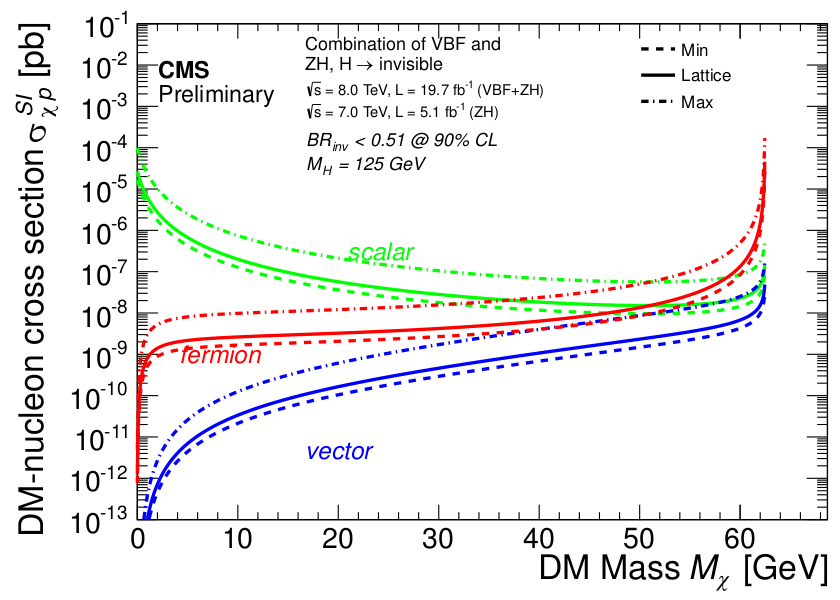
\includegraphics[width=\textwidth]{TalkPics/hig1330approval/dmlimit.png}
    \column{.5\textwidth}

    \footnotesize
    {\color{red} For approval as additional material}

    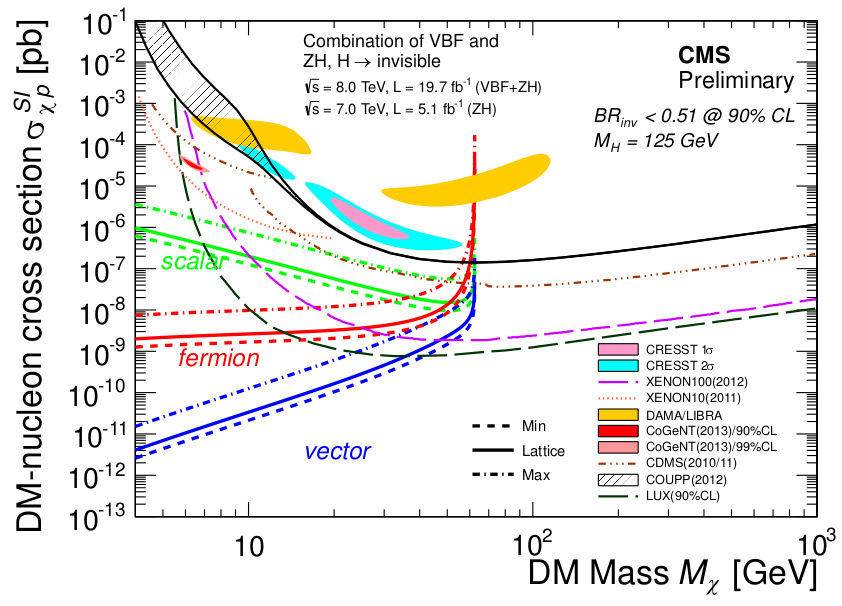
\includegraphics[width=\textwidth]{TalkPics/hig1330approval/dmlimitcontext.png}    
  \end{columns}
  \scriptsize
  \begin{block}{}
  \begin{itemize}
  \item $\mathcal{B}(H\rightarrow inv.)$ gives important exclusion in the low mass region
  \item Clearly we are only sensitive in the region $M_{\chi}<m_{h}/2$
  \end{itemize}
  \end{block}
\end{frame}

\begin{frame}
  \frametitle{Conclusions}
  \label{lastframe}
  \begin{columns}
    \column{.5\textwidth}
    \begin{block}{}
      \scriptsize
    \begin{itemize}
    \item All three H$\rightarrow$invisible channels have been combined using the standard Higgs combination tool
    \item The combined result gives the strongest limit on the invisible branching fraction of the 125 GeV Higgs [58(46)\%  Observed (expected) 95\% C.L. limit at 125 GeV]
    \item A Higgs portal dark matter interpretation of the above results has been presented and is particularly competitive at low mass
    \end{itemize}
    \end{block}
    \column{.5\textwidth}
    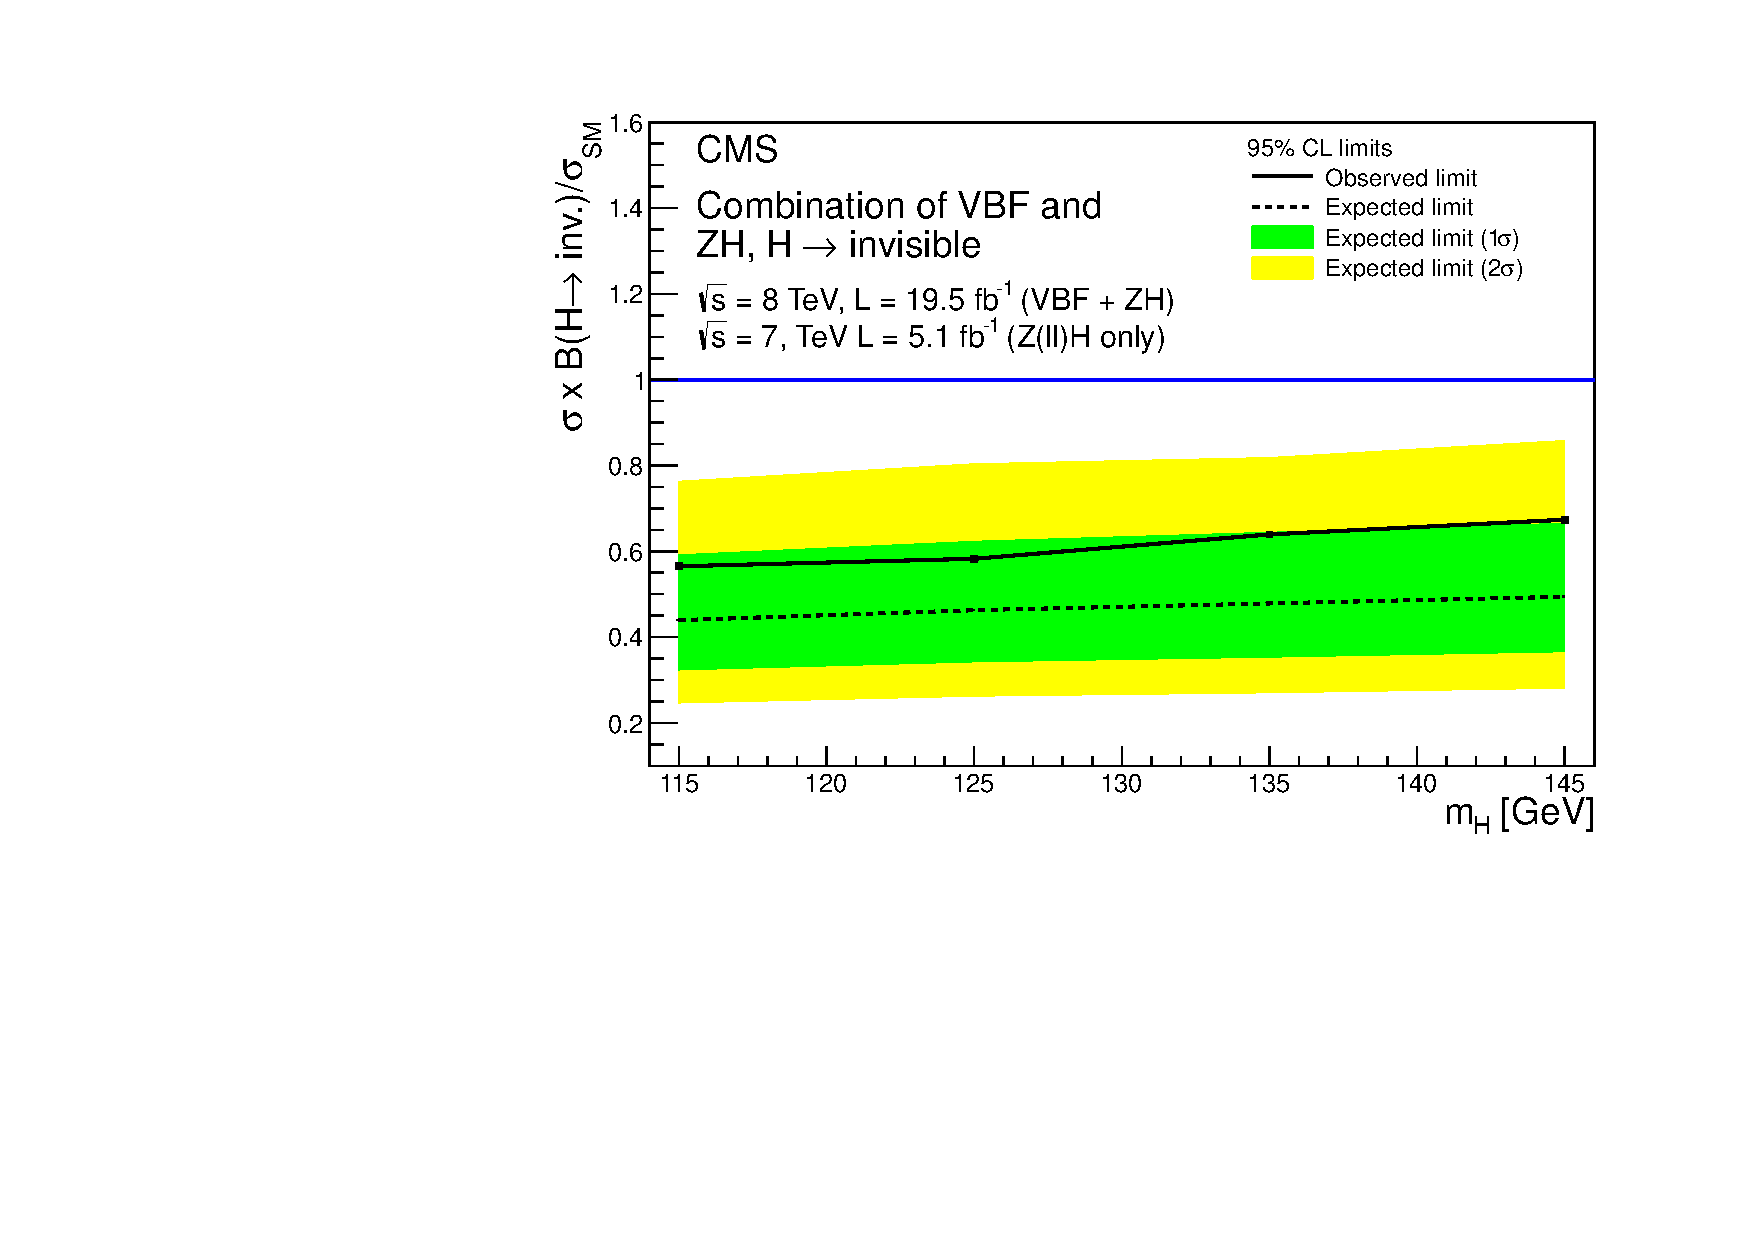
\includegraphics[clip=true,trim=0 0 0 0, width=1.1\textwidth]{TalkPics/hig1330approval/combinedlimit.pdf}
  
  \end{columns}
\end{frame}

\begin{frame}
  \frametitle{Backup}
\end{frame}

\begin{frame}
  \frametitle{Previous Limits}
  \begin{itemize}
  \item CMS PAS limits on $BR_{inv}$ for a 125 GeV Higgs boson are:
  \item[-] VBF: observed (expected) limit of 69\% (53\%) at 95\% C.L.
  \item[-] Z($\ell\ell$)H(inv): observed (expected) limit of 75\% (91\%) at 95\% C.L.
  \item[-] Z($b\bar{b}$)H(inv): ovserved (expected) limit of 182\% (199\%) at 95\% C.L.
  \item[-] CMS indirect limit, from visible channels: observed (expected) limit of 64\% (67\%) at 95\% C.L.
  \item ATLAS also produce an indirect limit and a limit in the ZH channel:
  \item[-] Indirect limit 60\% (no expected limit given)
  \item[-] ZH: observed (expected) 65\% (84\%)    
  \end{itemize}
\end{frame}

\begin{frame}
  \frametitle{VBF changes since PAS}
  \begin{block}{}
    \begin{itemize}
    \item New MC jet resolution measurement made at recommendation of JetMET
    \item ttbar cross-section updated from 234.0 $\rightarrow$ 245.8pb
    \item int. lumi changed from 19.576 $\rightarrow$ 19.494 $fb^{-1}$
    \item runMETuncertainty tool bug fixed
    \item lepton weights and ID efficiency uncertainties incorporated
    \item WGamma MC added
    \item Uncertainty correlations properly accounted for
    \item Plot cosmetics updated
    \end{itemize}
  \end{block}
\end{frame}

\begin{frame}
  \frametitle{Z(ll)H changes since PAS - presented to PAG 29/10/13}
    \begin{block}{}
      \scriptsize
      \begin{itemize}
      \item Original PAS (HIG-13-018) was based on two independent analyses:
      \item[-] AN-12-123, historically linked to ZZ analysis (SMP-12-016)
      \item[-] AN-13-148, historically linked to H$\rightarrow$WW analysis (HIG-13-003)
      \item These two analyses have been merged (AN-13-333):
      \item: Lepton ID, b-tagging taken from ZZ analysis
      \item: MET and M$_{T}$ definitions from WW analysis
      Additionally:
      \item A 1-jet bin has been added
      \item int. lumi has been updated
      \item Muon efficiency has been updated (3.5$\rightarrow$4.0\%)
      \item 2D shape analysis is used in limit setting for 8 TeV data
      \item A small change has been made to the data-driven Drell-Yan background
      \end{itemize}
    \end{block}
\end{frame}

\begin{frame}
  \frametitle{Z(ll)H changes since PAS continued - presented to PAG 29/10/13}
    \begin{block}{}
      \scriptsize
      \begin{itemize}
      \item $p_{T}$ dependent EW corrections added to ZH signal and WZ and ZZ backgrounds
      \item[-] ZH correction is taken from Z(bb)H(inv) analysis
      \item[-] WZ and ZZ correction parameterized from arxiv:1305.5402
      \item[-] Result - reduction in expected yields for both signal and background.
      \item[-] This is why observed limit increased (75$\rightarrow$83\%) even though expected limit decreased (91$\rightarrow$86\%)
      \item Generated additional signal mass points at 175, 200 and 300 GeV
      \end{itemize}
    \end{block}
\end{frame}

\begin{frame}
  \frametitle{Z(ll)H Final Limit Plots}
  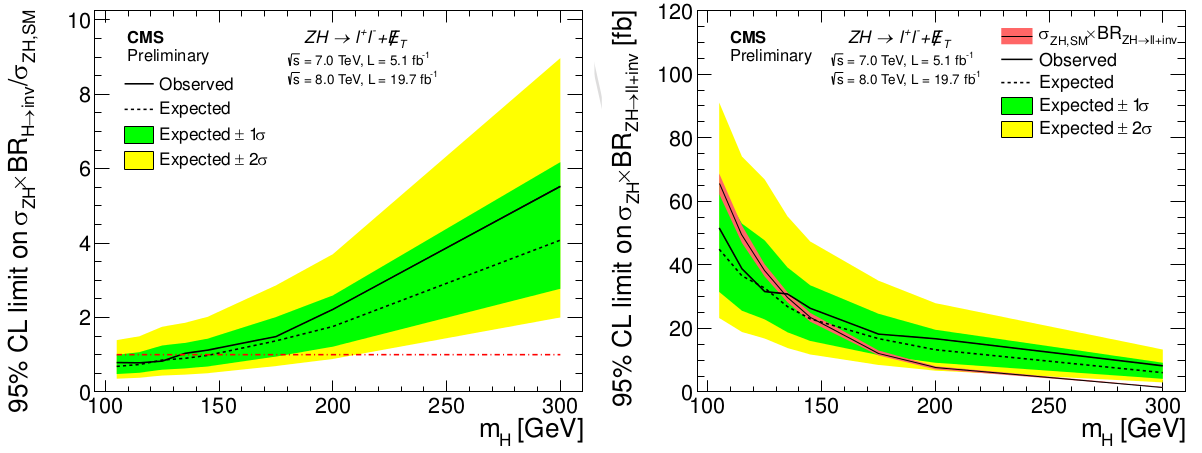
\includegraphics[width=\textwidth]{TalkPics/hig1330approval/zllfinallimitplots.png}%!!ADD FINAL ZLL PLOTS FROM AN
\end{frame}

\begin{frame}
  \frametitle{Z(bb)H changes since PAS}
  \begin{block}{}
    \scriptsize
    \begin{itemize}
    \item Apply EW corrections to VV backgrounds to be consistent with Z(ll)H(inv) (2-3\% changes to limits due to less background in high $p_{T}$ tails)
    \item Unified style and systematic naming with other two analyses
    \end{itemize}
  \end{block}
  \center
  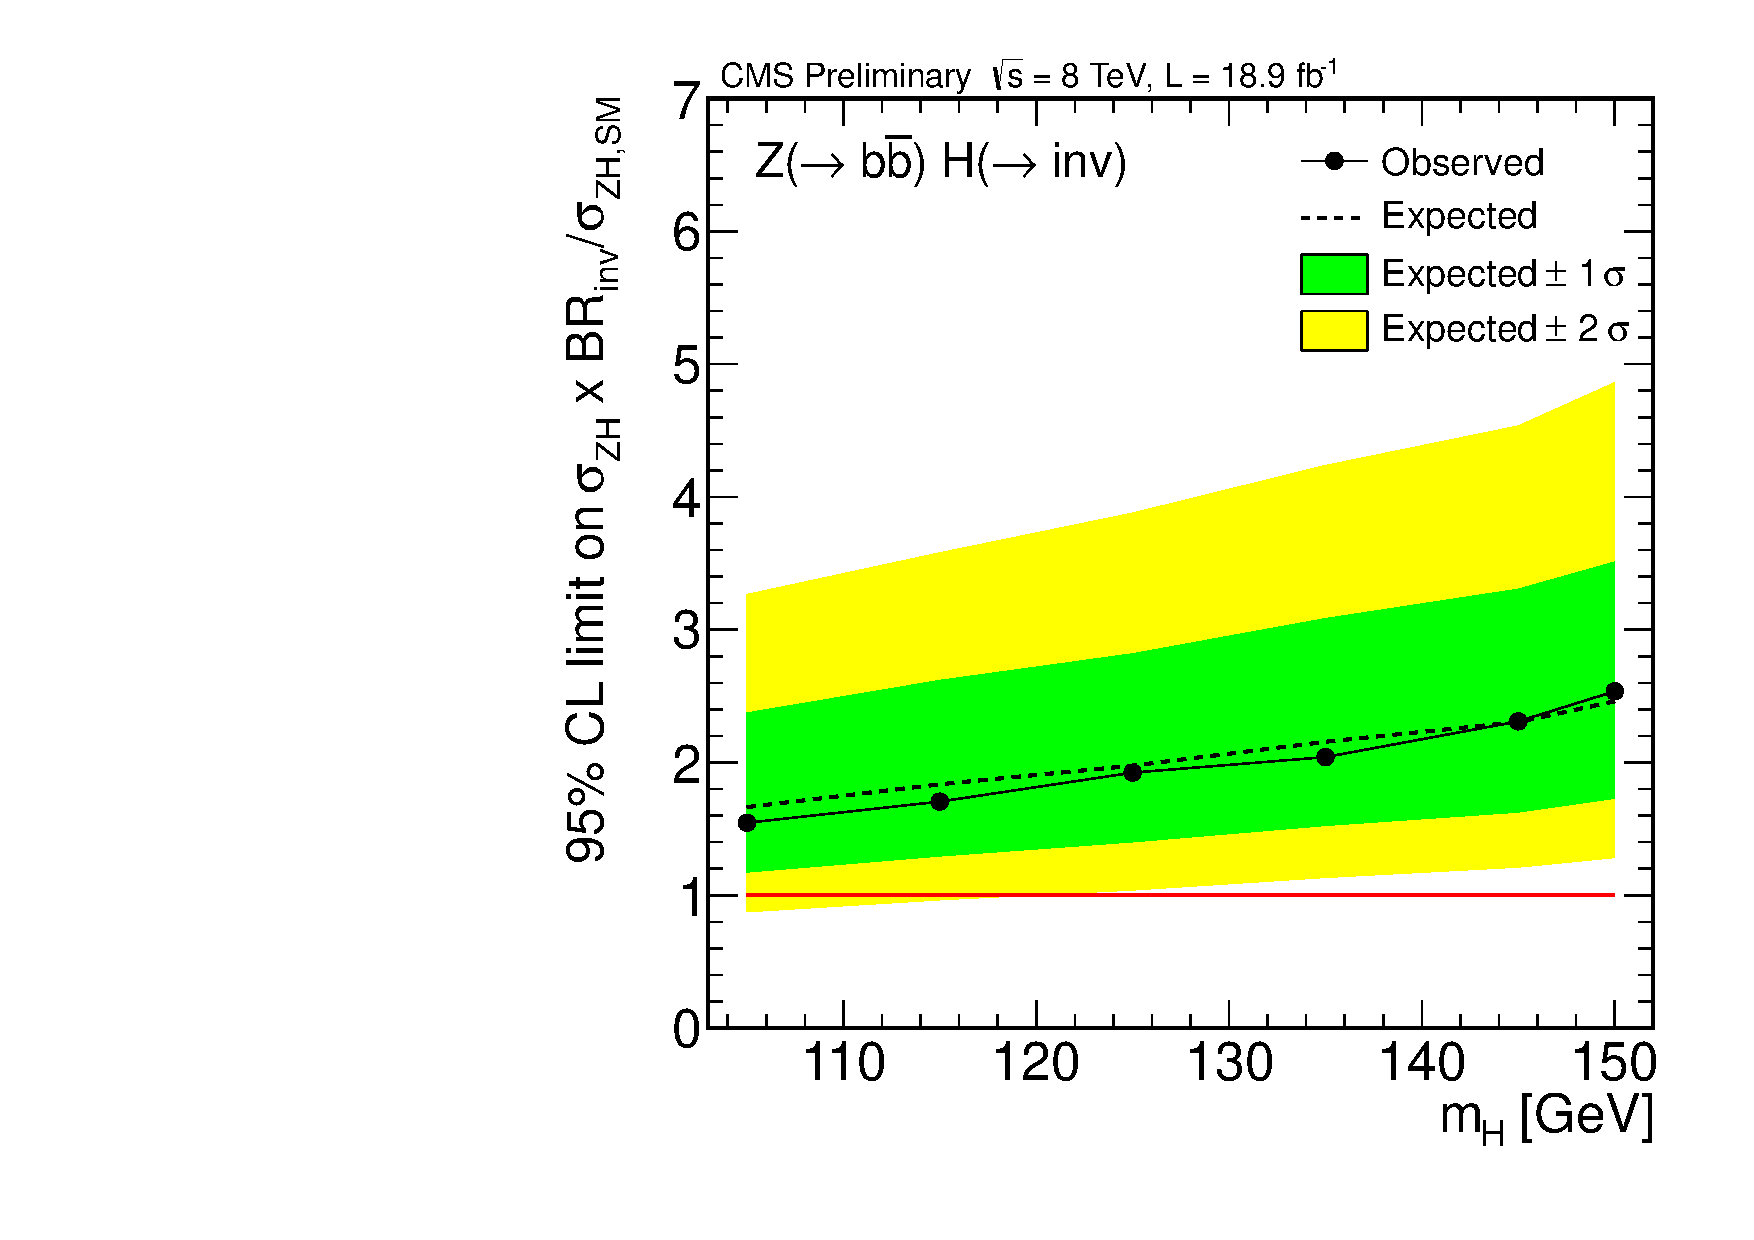
\includegraphics[width=.45\textwidth]{TalkPics/hig1330approval/zbboldlimit.pdf}
\end{frame}

\begin{frame}
  \frametitle{Values used for DM interpretation}
  \center
  \begin{block}{}
    \center
  \begin{tabular}{|l|c|}
    \hline
    Parameter & Value\\
    \hline
    $v$ &  174.0 GeV\\
    $m_{h}$ & 125.0 GeV\\
    $m_{N}$ & 938.95 MeV\\
    $\Gamma_{H}^{SM}$ & 4.07 MeV\\
    $f_{N}$ Lattice & 0.326\\
    $f_{N}$ Min & 0.260\\
    $f_{N}$ Max & 0.629\\
      \hline
  \end{tabular}
  \end{block}
  
\end{frame}



\begin{frame}
  \frametitle{VBF uncertainties by background}
  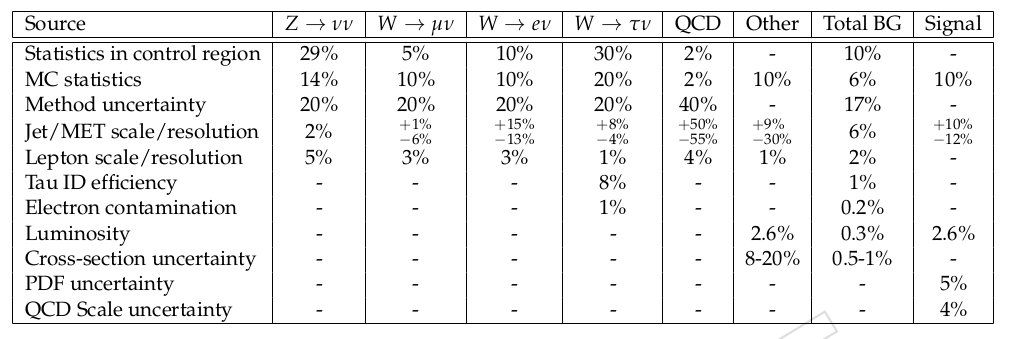
\includegraphics[width=\textwidth]{TalkPics/hig1330approval/vbfuncs.png}
\end{frame}

%% {
%% \setbeamercolor{background canvas}{bg=}
%% \includepdf[pages=31]{TalkPics/VBF-H-Invisible-Approval.pdf}
%% }

\end{fmffile}
\end{document}

